\documentclass[11pt]{standalone}

\usepackage{ifthen}
\usepackage{amsmath}
\usepackage{tikz} 
\usepackage[d]{esvect}
\usetikzlibrary{shapes.misc}
\usetikzlibrary{arrows,arrows.meta}
\usetikzlibrary{calc,intersections, patterns, math}

\definecolor{pfeil}{RGB}{168,167,167}
\definecolor{salmon}{RGB}{250,128,114}
\definecolor{petrol}{RGB}{0, 118, 136}
\definecolor{darkgoldenrod}{RGB}{184, 134, 11}
\colorlet{petrol-lighter}{petrol!40}
\colorlet{darkgoldenrod-lighter}{darkgoldenrod!40}

\begin{document}

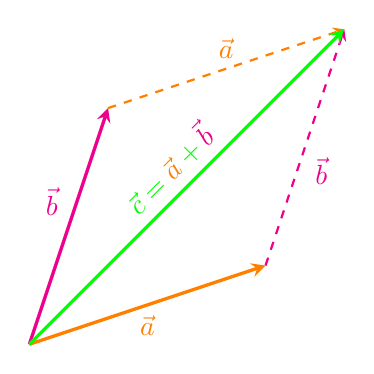
\begin{tikzpicture}[pfeil, >=stealth, very thick]
			
	\draw[orange,->] (1,1) -- node[below] {$\vec a$} (4,2);
	\draw[magenta,->] (1,1) -- node[above left] {$\vec b$} (2,4);
			
	\draw[magenta,dashed,thick,->] (4,2) -- node[below right] {$\vec b$} (5,5);
	\draw[orange,dashed,thick,->] (2,4) -- node[above]{$\vec a$} (5,5);
			
	\draw[green,->] (1,1) -- node[above, sloped] {$\vec c = {\color{orange}\vec a} + {\color{magenta}\vec b}$} (5,5);
\end{tikzpicture}			

\end{document}
